\chapter{Evaluatie van de proof-of-concept}
\label{ch:poc-evaluatie}

\section{Doel en onderzoeksvragen}

In Hoofdstuk \ref{ch:poc-implementatie} werd een PoC uitgewerkt om de ontbrekende schakel tussen Data\-bricks-ta\-bel\-len en Power BI-rap\-por\-ten zichtbaar te maken in OpenMetadata. Hierdoor ontstond een li\-ne\-age-ov\-er\-zicht op tabelniveau, gebaseerd op een generieke mappinglaag.\\

In dit hoofdstuk wordt deze PoC geëvalueerd vanuit het perspectief van rapportgebruikers, rapportbouwers en meer technische rollen bij VLAIO. De centrale vraag is in welke mate een expliciet overzicht van dataherkomsten, zoals gerealiseerd met OpenMetadata, bijdraagt aan het correct begrijpen en met vertrouwen gebruiken van rapporten. Zouden ze lineage, als gerealiseerd met de PoC effectief gebruke en hoe nuttig ervaren ze het? Bovendien dient de evaluatie om de grenzen van de huidige oplossing af te bakenen. In hoeverre volstaat dit overzicht op tabelniveau en welke praktische beperkingen ervaren gebruikers nog?\\

Meer concreet worden in dit hoofdstuk volgende evaluatievragen beantwoord:
\begin{itemize}
    \item \textbf{Validatie van het probleem:} In welke mate ervaren gebruikers vandaag inzicht in de herkomst van cijfers in rapporten, en hoe gaan zij om met wijzigingen of onduidelijkheden in data zonder expliciete lineage?
    \item \textbf{Validatie van de oplossing:} In welke mate helpt een visueel overzicht van de dataherkomst op tabelniveau om wijzigingen en hun impact op rapporten beter te begrijpen?
    \item \textbf{Rolspecifieke meerwaarde:} Verschilt de ervaren meerwaarde van zo'n overzicht tussen verschillende gebruikersprofielen, zoals rapportgebruikers, rapportbouwers en technische dataprofielen?
    \item \textbf{Beperkingen van de PoC:} Waar schiet de gerealiseerde lineage tekort en welke bijkomende informatie hebben gebruikers nog nodig?
    
\end{itemize}

Om deze vragen te beantwoorden werd een online vragenlijst afgenomen bij een selectie van VLAIO-medewerkers. De vragenlijst combineert enerzijds stellingen over de huidige ervaring zonder een expliciet inzicht in dataherkomst en anderzijds een scenario waarin een concreet herkomstoverzicht getoond wordt op basis van de gerealiseerde PoC. Daarna volgen er nog enkele vragen die enkel van toepassing zijn voor technische rollen en ten slotte een algemene evaluatie van de lineage.\\

\section{Onderzoeksopzet}

\subsection{Vragenlijst: Begrijpbaarheid en vertrouwen in rapporten}
De evaluatie maakt gebruik van een vragenlijst opgesteld in Microsoft Forms\footnote{Zie het volledige formulier in Bijlage~\ref{app:vragenlijst-begrijpbaarheid-vertrouwen}.}. Deze vragenlijst heeft als doel om inzicht te krijgen in hoe gebruikers rapporten interpreteren, omgaan met wijzigingen of onduidelijkheden in cijfers en in welke mate extra inzicht in dataherkomst daarbij kan helpen. De bevraging is anoniem, duurt ongeveer tien minuten en richt zich op een brede groep medewerkers die met rapporten werken. Op die manier is het mogelijk om inzichten te verzamelen vanuit verschillende perspectieven. Door de brede doelgroep werd de vragenlijst bewust toegankelijk gehouden. Technisch jargon zoals "lineage" of "impactanalyse" werd vermeden om de drempel voor eindgebruikers lager te houden en vertekende antwoorden te vermijden.\\

De vragenlijst is thematisch opgebouwd uit vijf blokken:
\begin{enumerate}
    \item \textbf{Profielvragen:} rol (rapportgebruiker, rapportbouwer, technisch dataprofiel), frequentie van rapportgebruik en zelfgerapporteerde vertrouwdheid met de onderliggende data.
    \item \textbf{Huidige ervaring zonder extra inzicht:} Likert-schalen (1--5) rond zicht op de herkomst van cijfers, het kunnen verklaren van wijzigingen en het inschatten van impact op andere rapporten, aangevuld met een open vraag naar een concrete situatie waarin men twijfelde aan de cijfers of hun herkomst.
    \item \textbf{Scenario met herkomstoverzicht:} introductie van een vereenvoudigde visualisatie van de lineageketen van databronnen tot een rapport, gevolgd door stellingen over begrijpelijkheid, bruikbaarheid en impact op vertrouwen.
    \item \textbf{Extra vragen voor technische profielen:} bijkomende stellingen voor rapportbouwers en technische dataprofielen over de rol van zo'n overzicht bij impactanalyses en het onderbouwen van wijzigingen.
    \item \textbf{Algemene evaluatie:} algemene stellingen over de meerwaarde en het verwachte gebruik van een herkomstoverzicht, plus een optionele open vraag.
\end{enumerate}

De meeste gesloten vragen maken gebruik van een vijfpuntsschaal (van 'helemaal oneens' tot 'helemaal eens'). Dit laat toe om zowel een beschrijvend beeld te schetsen van de huidige situatie, als om de ervaren meerwaarde van het herkomstoverzicht hiermee kwantitatief te vergelijken. De open vragen bieden daarnaast ruimte voor wat meer nuance en concrete voorbeelden.\\

\subsection{Scenario en visualisatie van dataherkomst}

In het derde blok van de vragenlijst wordt de PoC expliciet in beeld gebracht via een vereenvoudigde visualisatie van de lineageketen. De respondenten krijgen hier een schematische weergave te zien waarin links de databronnen en tussenliggende datastappen staan en rechts het rapport dat met deze data gevoed wordt. De verbindingen tonen welke datasets doorstromen naar het rapport, gebaseerd op de in OpenMetadata vastgelegde relaties op tabelniveau.\\

De introductietekst bij deze representatie van lineage legt uit dat het overzicht automatisch wordt opgebouwd op basis van metadata en dat het toelaat om bij een wijziging in één van de datasets na te gaan welke rapporten en cijfers hierdoor geraakt kunnen worden. Op die manier wordt de PoC in een realsitische en herkenbare situatie geplaatst, zodat gebruikers kunnen duidelijk maken in welke mate zo’n overzicht hen zou helpen om wijzigingen en hun impact beterte begrijpen. Daarnaast kan ook worden nagegaan of de gerealiseerde scope, namelijk een herkomstoverzicht op tabelniveau, in de praktijk voldoende detail biedt om nuttig te zijn voor de verschillende gebruikers.\\

\section{Resultaten}

\subsection{Profiel van de respondenten}
Op het moment van analyse hebben 24 respondenten de vragenlijst volledig ingevuld. Dit biedt een eerste indruk op waar de grootste uitdagingen liggen, wat er nodig is om rapporten beter te kunnen interpreteren en hoe lineage hierop inspeelt.\\

De steekproef bestaat uit 7 rapportgebruikers, 8 occasionele rapportbouwers en 9 technische dataprofielen, wat een goede mix van de verschillende rollen is(zie Figuur~\ref{fig:verdeling}). Daarnaast blijkt uit de gebruiksfrequentie (Figuur~\ref{fig:frequentie}) dat 21 van de 24 respondenten dagelijks of wekelijks met rapporten werkt. Deze hoge betrokkenheid versterkt de relevantie van hun feedback binnen VLAIO.

\begin{figure}[H]
    \centering
    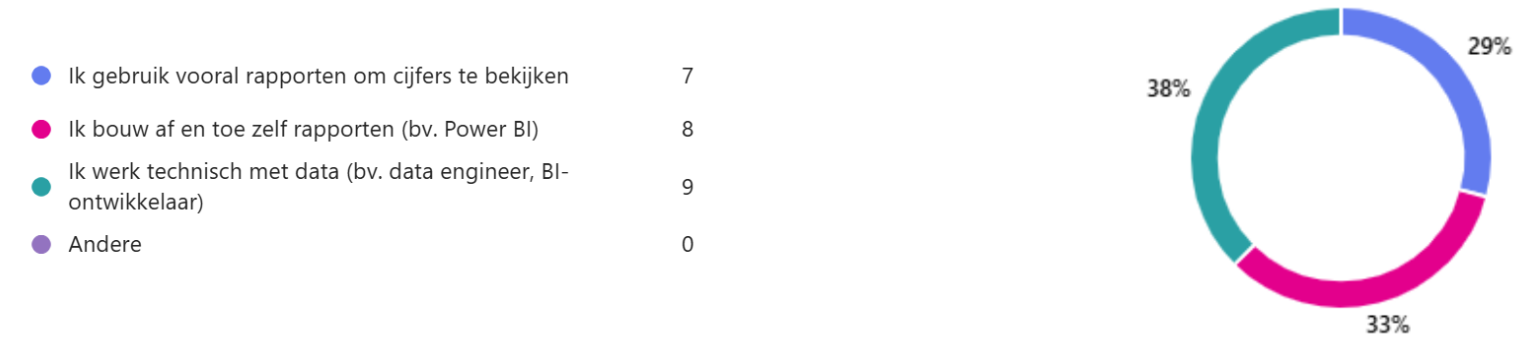
\includegraphics[width=0.8\textwidth]{images/verdeling.png}
    \caption{Verdeling van de respondenten over de verschillende professionele profielen binnen VLAIO.}
    \label{fig:verdeling}
\end{figure}

\begin{figure}[H]
    \centering
    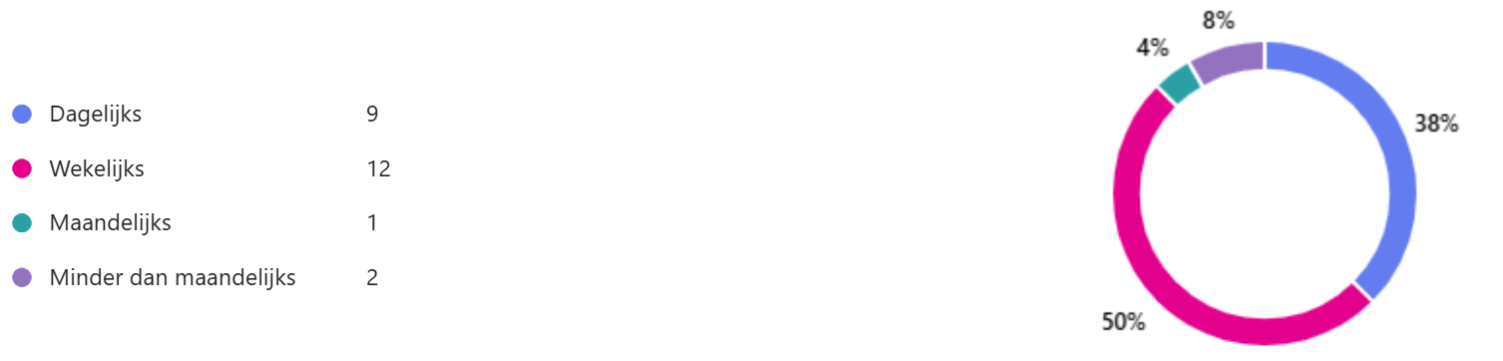
\includegraphics[width=0.8\textwidth]{images/frequentie.png}
    \caption{Frequentie van rapportgebruik onder de respondenten. Het overgrote deel (88\%) werkt op dagelijkse of wekelijkse basis met rapporten.}
    \label{fig:frequentie}
\end{figure}

\subsection{Huidige ervaring zonder expliciet inzicht in dataherkomst}

De antwoorden op de stellingen over de huidige situatie tonen een dubbel beeld. Hoewel een ruime meerderheid (83,3\%) aangeeft doorgaans goed te weten waar rapportcijfers vandaan komen, blijkt het dat het daadwerkelijk verklaren van wijzigingen en het inschatten van de impact ervan een stuk uitdagender is. Bijna een vijfde (~17\%) van de respondenten heeft moeite om te bepalen welke andere rapporten of processen door een aanpassing geraakt worden. Dit bevestigt dat het zicht op de onderlinge afhankelijkheden binnen de dataketen vandaag sterk beperkt is, zelfs bij de meer technisch profielen.\\

De open antwoorden verduidelijken dat deze onzekerheid zelden voortkomt uit twijfel over het rekenwerk zelf. Het komt vooral uit een gebrek aan semantische transparantie en context. Respondenten geven aan dat rapporten die zij niet zelf gebouwd hebben, vaak als minder betrouwbaar aanvoelen. Doordat ze hier zelf niet aan werkten, is het soms onduidelijk welke filters, aggregaties of definities precies zijn gebruikt. Zo is de naamgeving in Power BI vaak anders dan in een bronsysteem of is het niet meteen helder of een cijfer over "toegekende" of "finaal uitbetaalde" steun gaat. Een voorbeeld uit de bevraging illustreert dit goed. Een schijnbare daling in de 'doorlooptijd' van dossiers bleek niet het gevolg van snellere verwerking, maar van een ongedocumenteerde verandering van een definitie in het rapport. Zonder expliciete metadata is het voor een eindgebruiker nagenoeg onmogelijk om te achterhalen of een veranderd cijfer voortkomt uit de brondata, een aangepaste definitie of een ontwerpfout.\\

Opvallend is dat dit probleem zich niet beperkt tot zakelijke eindgebruikers. Ook technische profielen geven aan dat het begrijpen van datastromen en het traceren van wijzigingen een aanzienlijke uitdaging vormt. Eén respondent stelt: "Het duurt heel lang voor je een dataset door en door kent. Zelfs na jaren ermee te werken kan er plots iets opduiken wat je niet had verwacht na een change." Volgens een andere respondent is het moeilijk voor een analist om cijfers te verifiëren wanneer deze enkel "fragmentarische kennis van de data" heeft en het achterliggend bronsysteem niet goed kent. Dit toont aan dat de complexiteit van datastromen niet enkel voor eindgebruikers een barrière vormt. Ook ontwikkelaars verliezen kostbare tijd aan het handmatig onderzoeken van afhankelijkheden.\\

Samengevat hebben verschillende profielen moeite met het opvolgen van wijzigingen en het begrijpen van de achterliggende definities. Van alle respondenten zegt 70,8\% dat die meer vertrouwen in de cijfers zou hebben als de oorsprong beter zichtbaar was. Dit toont duidelijk aan dat een er brede een brede behoefte aan inzichtelijke data lineage is.\\

\subsection{Ervaren meerwaarde van het lineage-overzicht}
Na het tonen van de visualisatie van lineage wordt het overzicht overwegend positief beoordeeld als hulpmiddel voor traceerbaarheid en impactanalyse. Ronduit 75,0\% van de respondenten geeft aan dat het hen helpt om sneller te zien waar cijfers vandaan komen. Ook het inschatten van de impact bij wijzigingen wordt als duidelijker ervaren. Ongeveer zeventig percent gaat ermee akkoord dat het overzicht helpt om beter in te schatten welke onderdelen of rapporten door een wijziging geraakt worden. Tegelijk scoort "meer vertrouwen in de data door het overzicht" merkelijk lager. Slechts 54,2\% gaat akkoord en 25,0\% is het er expliciet mee oneens. Dit geeft dat traceerbaarheid en vertrouwen niet automatisch samengaan.\\

De gedetailleerde resultaten van deze stellingen zijn weergegeven op Figuur \ref{fig:stellingen}:\\
\begin{figure}[H]
    \centering
    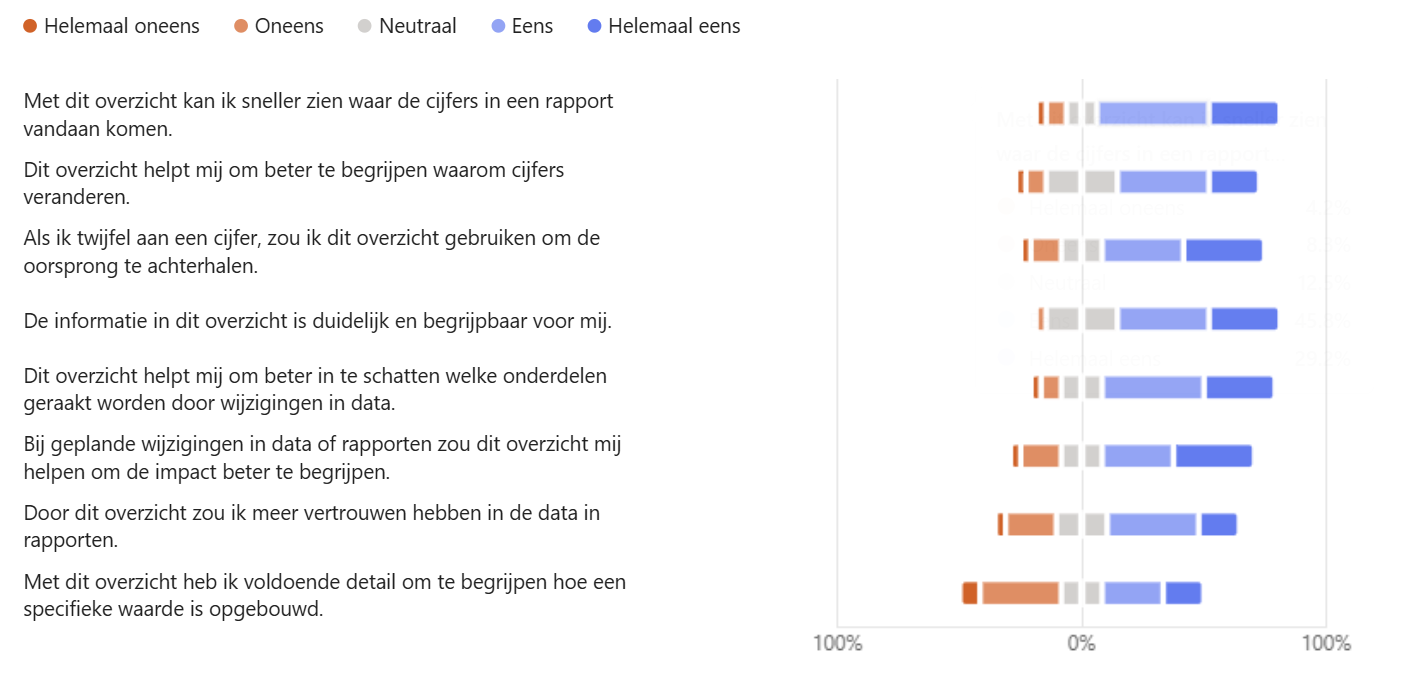
\includegraphics[width=\textwidth]{images/lineage_stellingen.png}
    \caption{Mate waarin respondenten akkoord gaan met stellingen over de meerwaarde en het gebruik van het getoonde lineage-overzicht ($n=24$).}
    \label{fig:stellingen}
\end{figure}

Deze resultaten tonen dat een visuele voorstelling van dataherkomst, zoals gerealiseerd met de PoC, al een bruikbaar vertrekpunt vormt om de eerder vastgestelde zichtbaarheidskloof te overbruggen. Toch toont de bevraging dat deze meerwaarde niet volledig is. Op de stelling of het overzicht voldoende detail biedt om te begrijpen hoe een specifieke waarde is opgebouwd, gaat slechts 41,7\% akkoord, terwijl een even grote groep (41,7\%) hier expliciet mee oneens is. Respondenten vinden verbanden makkelijker terug dankzij de visualisatie, maar begrijpen nog steeds niet hoe de cijfers precies zijn samengesteld. Dat bevestigt de lage score op die vraag.\\

De open antwoorden illustreren deze grens. Meerdere personen geven aan dat het getoonde overzicht te generiek blijft en onvoldoende detail bevat om te begrijpen hoe specifieke waarden precies zijn opgebouwd. Ze willen weten welke kolommen eronder zitten, wat specifieke datavelden juist inhouden, welke regels er werden toegepast en hoe samengevoegde cijfers tot stand komen. Zo stelde één respondent: "je hebt nu enkel bronnen, maar je weet niet hoe data binnen een bepaalde bron is opgebouwd." Een andere formuleerde het breder: "er is geen beschrijving van bronsysteem, zijn werking en inherente logica, ETL, aanwezige businesslogica en andere details." Daarnaast missen ze informatie over hoe actueel de data is en wat bepaalde technische begrippen precies betekenen. Zonder dat is het lastig om veranderingen op de juiste manier te kunnen interpreteren.\\

Daarbij valt ook duidelijk een verschil op in de noden van de verschillende groepen van profielen. Technische profielen zien het overzicht als een handig, oriënterend startpunt, maar vinden het te beperkt voor een grondige analyse uit te voeren. Ze willen ook inzicht in de ETL-logica, de toegepaste transformaties en hoe modellen zijn opgebouwd. Daarbij is wel belangrijk om te nuanceren dat er binnen de bestaande lineage in OpenMetadata voor eerdere delen van de dataketen wél al bijkomend detail beschikbaar kan zijn. Voor bepaalde tabellen kan vanuit de lineage immers worden doorgeklikt naar de achterliggende SQL-query of datatransformatie, waardoor de verwerking gedeeltelijk zichtbaar wordt. Deze mogelijkheid ontbreekt echter voor de specifieke schakel tussen platinum-datasets en Power BI-rapporten, die net centraal staat in deze PoC.\\

Bij minder technische gebruikers ligt de beperking anders. Daar blijkt uit de open antwoorden dat het overzicht soms als te abstract wordt ervaren. Voor deze groep volstaat een visueel overzicht van databronnen en tabellen niet altijd om cijfers echt beter te begrijpen, tenzij het gekoppeld wordt aan een meer toegankelijke toelichting, duidelijke business definities of doorklikmogelijkheden vanuit het rapport. Een respondent verwoordt deze voorwaarde helder: \textit{"Naast de definitie in SQL of Python kunnen terugvinden, is het voor de meeste eindgebruikers belangrijk om de gedefinieerde waarden ook in business-taal te kunnen raadplegen. Voor het vertrouwen is dus niet enkel die herkomst van belang, maar ook correcte definities."}.\\

De respondenten zijn zeker wel geinteresseerd in de lineage: 87,5\% vindt dat het overzicht helpt om rapporten beter te begrijpen, en 83,3\% zou het nuttig vinden als rapporten standaard een link bevatten naar zo'n overzicht. Geen enkele respondent beoordeelt dit als onnuttig. Dat toont dat gebruikers een duidelijke eerste meerwaarde erkennen. Het stelt gebruikers in staat om sneller betrokken datasets en rapporten te identificeren en de initiële impact van wijzigingen breder vast te leggen. Toch wijst de bevraging naar waar de gerealiseerde PoC tekortkomt. Een overzicht op tabelniveau volstaat echter niet om de semantische betekenis en de transformatielogica achter de cijfers te verklaren. Dit onderstreept dat een visuele keten pas echt de volledige onzekerheid wegneemt wanneer technische lineage verder verfijnd kan worden (bijvoorbeeld tot op kolomniveau) en gekoppeld wordt aan heldere, toegankelijke business-definities.\\

\subsection{Impact op vertrouwen en toekomstig gebruik}

Uit de bevraging blijkt een duidelijke bereidheid om lineage structureel te integreren in het dagelijkse werk. Een ruime meerderheid (66,7\%) geeft aan het overzicht effectief te zullen raadplegen bij twijfel over cijfers. Er is ook brede steun voor het idee om rapporten standaard te voorzien van een rechtstreekse link naar hun dataherkomst in OpenMetadata (zie Figuur~\ref{fig:vertrouwengebruik}).\\

\begin{figure}[H]
    \centering
    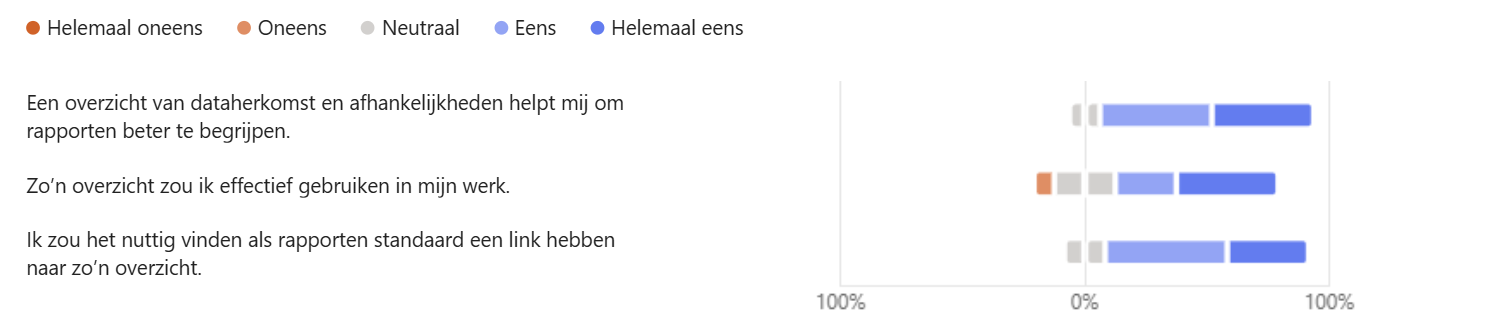
\includegraphics[width=\textwidth]{images/vertrouwen_gebruik.png}
    \caption{Mate waarin respondenten akkoord gaan met stellingen over de impact van lineage op vertrouwen en het toekomstig gebruik.}
    \label{fig:vertrouwengebruik}
\end{figure}

Het valt op dat gebruikers die aangeven minder vertrouwd te zijn met de onderliggende data, de hoogste verwachtingen hebben van lineage om hun vertrouwen te versterken. Dit is zeker begrijpelijk. Zij staan het verst van de bron en hebben dus het meeste voordeel bij een centraal overzicht van dataherkomst. De antwoorden tonen echter wel dat lineage voor deze groep pas echt waardevol wordt wanneer de technische herkomst gecombineerd wordt met begrijpelijke uitleg. Zoals eerder vermeld volstaat een puur technisch overzicht met abstracte tabelnamen op OpenMetadata niet. Zonder context over wat die tabellen betekenen, blijft het voor niet-tech\-ni\-sche gebruikers moeilijk om dit te interpreteren. Respondenten geven dan ook aan dat ze vanuit het lineage-overzicht vlot willen kunnen doorklikken naar businessdefinities of bijkomende toelichting over de betekenis van de getoonde data.\\ 

\subsection{Verschillen tussen gebruikersprofielen}

Er is dus een duidelijk verschil te zien in hoe de verschillende profielen naar lineage kijken. Respondenten die zelf rapporten bouwen of technisch met data werken, zien de PoC voornamelijk als een tool voor communicatie en analyse. Deze groep scoort opvallend hoog op de stelling dat het overzicht hen helpt om impactanalyses beter te onderbouwen naar anderen (zie Figuur \ref{fig:analyseimpact}). Tegelijkertijd voelt precies deze groep de beperkingen van de PoC het sterkst. Zij hebben bijkomend detail nodig over de exacte kolommen en de achterliggende transformaties om wijzigingen daadwerkelijk door te kunnen voeren of debuggen. Voor daadwerkelijke probleemoplossing grijpen zij toch terug naar de ruwe data. Zoals een data-engineer aangeeft: \textit{"Met een test-attitude probeer ik enkele gevallen van data tot rapport [...], dan pas verdwijnt de twijfel."} Het grafische overzicht volstaat voor hen dus niet als pure analysetool. Bij deze groep heeft het als tool voor communicatie wel zijn waarde. Het dient daarbij als een gedeeld referentiekader om de impact van wijzigingen begrijpelijk te maken voor stakeholders met een mindere technische achtergrond.

\begin{figure}[H]
    \centering
    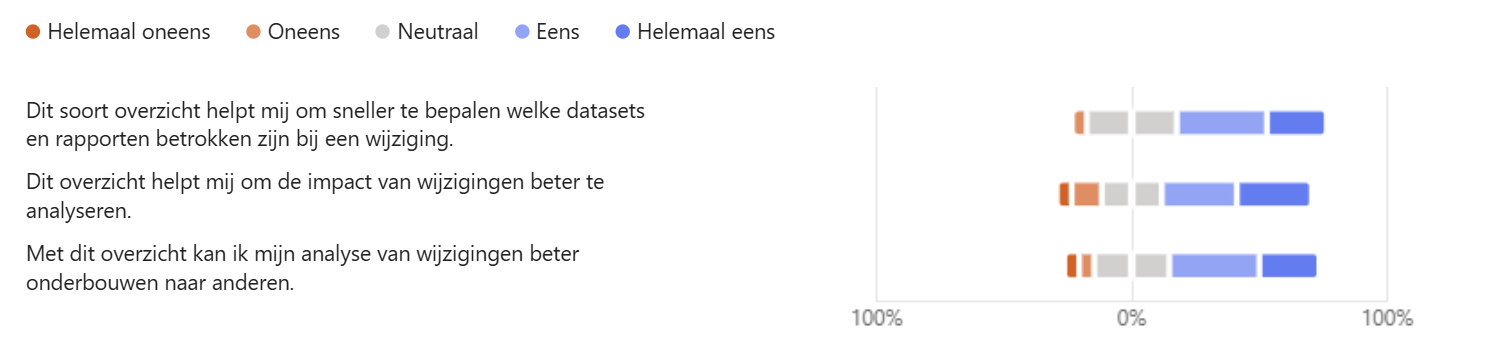
\includegraphics[width=\textwidth]{images/analyse_impact.png}
    \caption{Mate waarin respondenten akkoord gaan met stellingen over de ondersteuning bij impactanalyses en het onderbouwen van wijzigingen.}
    \label{fig:analyseimpact}
\end{figure}

Rapportconsumenten focussen bij de bevraging veel meer op begrijpbaarheid. Voor hen is lineage vooral nuttig om sneller te zien waar cijfers vandaan komen en waarom ze veranderen. Zoals eerder vermeld geven ze wel aan dat de schema's te abstract zijn. Zo stelt een eindgebruiker letterlijk dat tabelnamen en datastromen voor hen \textit{"abstracte concepten"} blijven. Voor rapportconsumenten is een data lineage-tool op tabelniveau dus pas waardevol wanneer het wetkt als een betrouwbaar navigatiemiddel richting de juiste, men\-sen\-taal-do\-cu\-men\-ta\-tie, en niet als een opzichzelfstaand overzicht.\\

Voor technische profielen en bouwers ondersteunt lineage dus in de eerste plaats het identificeren van betrokken datasets en het structureren van impactanalyses over teams heen. Voor niet-technische consumenten vormt het voornamelijk een tool om de herkomst van cijfers en de aard van wijzigingen beter te begrijpen.

\section{Synthese met aanbevelingen}

Deze evaluatie bevestigt het beeld dat in de contextanalyse (Hoofdstuk~\ref{ch:contextanalyse}) en de stand van zaken (Hoofdstuk~\ref{ch:stand-van-zaken}) werd geschetst. De zichtbaarheid van de laatste stap in de dataketen, van platinum-dataset naar rapport, blijkt in de praktijk een reëel knelpunt. Zonder expliciet inzicht in dataherkomst en afhankelijkheden hebben zowel rapportconsumenten als technische profielen moeite om wijzigingen correct te interpreteren, definities eenduidig te houden en de impact van veranderingen in te schatten. De bevraging toont dat 70{,}8\% van de respondenten meer vertrouwen zou hebben in de cijfers als de oorsprong beter zichtbaar is, terwijl 75{,}0\% aangeeft dat het getoonde herkomstoverzicht effectief helpt om sneller te zien waar data vandaan komt en welke rapporten door wijzigingen geraakt worden.

Tegelijkertijd markeren de resultaten scherp de grenzen van de gekozen aanpak. Een overzicht op tabelniveau volstaat als eerste laag om betrokken datasets en rapporten te identificeren, maar niet om de opbouw van individuele waarden of de semantische betekenis van cijfers volledig te doorgronden. Slechts 41{,}7\% van de respondenten vindt dat het overzicht voldoende detail biedt om te begrijpen hoe een specifieke waarde is samengesteld, terwijl een even grote groep het hiermee expliciet oneens is. In de open antwoorden wordt herhaaldelijk verwezen naar \emph{fragmentarische kennis van de data} en naar het feit dat men zonder toegang tot de volledige keten van bron tot rapport moeilijk kan nagaan waar een probleem juist ontstaat. Dit sluit nauw aan bij de literatuur rond data governance, waar technische lineage pas als volwaardige analysetool wordt beschouwd wanneer zij wordt aangevuld met een semantische laag en meer detail.

Op basis van deze bevindingen kunnen voor VLAIO een aantal concrete vervolgstappen worden geformuleerd.

\subsection*{Aanbeveling 1: Uitbouw naar kolomniveau en automatische SQL-opvang}

De huidige PoC maakt de afhankelijkheden tussen platinum-tabellen en Power~BI-rapporten zichtbaar op tabelniveau. Verschillende respondenten geven echter aan dat echte impactanalyse pas mogelijk wordt wanneer duidelijk is welke kolommen en berekeningen in een rapport gebruikt worden. Een eerste aanbeveling is dan ook om de technische lineage verder uit te bouwen naar kolomniveau, door SQL-queries en transformaties langs in OpenMetadata systematisch op te vangen en te koppelen aan de bijhorende rapporten.

Concreet betekent dit dat er kan onderzocht worden of met de bestaande functionaliteiten van OpenMetadata en Databricks, het mogelijk is om query's te analyseren en kolom-af\-han\-ke\-lijk\-he\-den af te leiden. Dit kan door:
\begin{itemize}
	\item SQL-statements uit notebooks, jobs of views op te vangen en via de OpenMetadata-ingestie te laten parsen naar kolomlineage;
	\item duidelijke naamgevingsconventies af te spreken voor views en transformaties (bijvoorbeeld \texttt{\textless domein\textgreater\_\textless laag\textgreater\_\textless onderwerp\textgreater}), zodat deze in SQL, Databricks en OpenMetadata op een consistente manier herkenbaar en herleidbaar blijven;
	\item waar Power BI-rapporten expliciete DAX- of query-definities bevatten, te onderzoeken in welke mate deze informatie voor aanvullende lineage kan worden gebruikt.
\end{itemize}

Indien deze stap wordt gerealiseerd, evolueert OpenMetadata van een oriënterend overzicht naar een vrijwel volledige analysetool. Voor veel vragen rond wijzigingen en impact wordt het dan niet langer nodig om in notebooks en code te duiken of domeinkennis bij collega’s te zoeken. Alle impact kan dan rechtstreeks vanuit de metadata worden afgeleid. Dat sluit aan bij de eerder vermelde situaties die respondenten beschrijven, waarin onverwachte effecten na een change vaak pas na intensief speurwerk aan het licht komen. Met een volledig lineage op kolomniveau, als zichtbare onderliggende transformaties, zullen situaties als deze niet meer het geval zijn.

\subsection*{Aanbeveling 2: Koppeling met businesslogica en definities}

Voor rapportconsumenten is technische lineage op zich onvoldoende om cijfers echt beter te begrijpen. In de bevraging wordt meermaals benadrukt dat  ook een duidelijke uitleg in bu\-si\-ness-taal nodig is om cijfers correct te interpreteren. Dit speelt eveneens bij technische profielen wanneer definities wijzigen, zoals geïllustreerd in het voorbeeld rond de veranderde definitie van doorlooptijd.\\

Een tweede aanbeveling is daarom om de bestaande lineage expliciet te koppelen aan businesslogica. OpenMetadata biedt hiervoor concrete functionaliteit, onder meer via:
\begin{itemize}
	\item \textbf{Glossaries en business-termen:} voor kernbegrippen zoals \emph{toegekende steun}, \emph{finaal uitbetaalde steun} of \emph{doorlooptijd} kunnen formele definities worden vastgelegd en gekoppeld aan de relevante tabellen en kolommen;
	\item \textbf{Beschrijving en tags op veldniveau:} belangrijke velden in platinum-tabellen en rapporten kunnen worden verrijkt met een korte beschrijving in begrijpbare taal en, waar nodig, met verwijzingen naar beleidsdocumenten of rekenregels;
	\item \textbf{Versiebeheer van definities:} wanneer definities wijzigen, kan dit via metadata zichtbaar worden gemaakt, zodat duidelijk blijft vanaf wanneer een cijfer volgens een nieuwe logica wordt gerapporteerd.
\end{itemize}

Voor eindgebruikers ontstaat zo een doorstroom van rapport naar herkomst met betekenis. Deze kan dan van een waarde in Power BI via de lineage naar de onderliggende tabel en vervolgens naar een businessdefinitie die in gewone taal uitlegt wat het cijfer precies voorstelt. Dit zou de misverstanden die in de bevraging aan bod kwamen bijvoorbeeld rond verschillen tussen toegekende en uitbetaalde steun, of tussen oude en nieuwe definities van doorlooptijd, grotendeels kunnen voorkomen.\\

\subsection*{Aanbeveling 3: Inbedden van lineage in change- en releaseproces}

De resultaten tonen aan dat veel problemen rond vertrouwen ontstaan wanneer wijzigingen in bronnen, boekhoudsleutels of definities niet tijdig of onvoldoende transparant gecommuniceerd worden.\footnote{Zie bijvoorbeeld respondent 15 over wijzigingen in bronsystemen en respondent 23 over veranderende allocaties van fondsen.} Een derde aanbeveling is daarom om het gebruik van lineage niet louter als technische voorziening te zien, maar het expliciet te verankeren in het change- en releaseproces.\\

Binnen VLAIO bestaan vandaag al impactanalyse-documenten, waarin een sectie voorzien is voor lineage. De evaluatie suggereert dat deze sectie nog niet systematisch gevoed wordt met actuele metadata uit OpenMetadata.

ogelijke concrete stappen zijn:
\begin{itemize}
	\item bij wijzigingen in bronsystemen, platinum-tabellen of kernrapporten systematisch na te gaan — via OpenMetadata — welke datasets en rapporten geraakt worden, en deze lijst te gebruiken als basis voor communicatie naar stakeholders;
	\item bij grotere wijzigingen in kernmodellen het bestaande impactanalyse-document verplicht te laten verwijzen naar een relevante lineage-view in OpenMetadata, of een beknopte impactanalyse op basis van die lineage in de voorziene sectie te documenteren;
	\item de bestaande Databricks-jobs voor lineage-opbouw in te plannen volgens de ritmes van bron- en rapportvernieuwing, zodat het overzicht actueel blijft en change-analyses steeds op recente metadata gebaseerd zijn.
\end{itemize}

Op die manier verschuift lineage van een louter ondersteunende PoC naar een vast onderdeel van de manier waarop wijzigingen binnen de data-omgeving van VLAIO worden gepland, uitgevoerd en opgevolgd, met expliciete verankering in de bestaande impactanalyse-documenten.

\subsection*{Aanbeveling 4: Toegankelijke toegangspunten voor rapportconsumenten}

Tot slot tonen de resultaten dat de bereidheid om lineage te gebruiken groot is, 66{,}7\% zou het overzicht effectief raadplegen bij twijfel en veel respondenten vinden een standaardlink vanuit het rapport wenselijk -- maar dat de huidige weergave voor sommige gebruikers te technisch en abstract blijft.
Een vierde aanbeveling is daarom om voor rapportconsumenten één of meerdere toegankelijke toegangspunten te voorzien:

Mogelijke concrete invullingen zijn:
\begin{itemize}
	\item een vereenvoudigde, gefilterde lineage-view per rapport, waarin enkel de relevante deelketen wordt getoond, aangevuld met een korte tekstuele toelichting in begrijpbare taal;
	\item duidelijke richtlijnen of een korte handleiding waarin stap voor stap wordt uitgelegd hoe gebruikers het juiste rapport in OpenMetadata kunnen terugvinden op basis van de rapportnaam in Power~BI;
	\item waar nodig, begeleidende documentatie, een korte opleidingssessie of uitlegpagina's met screenshots die tonen hoe lineage gelezen kan worden en hoe businessdefinities aan tabellen en velden gekoppeld zijn.
\end{itemize}

Op die manier blijft dezelfde technische basis (OpenMetadata en de PoC) behouden, maar wordt de drempel voor niet-technische gebruikers verlaagd en sluit de toepassing beter aan bij hun verwachtingen rond begrijpelijkheid en vertrouwen. Een eventuele directe link vanuit kritieke rapporten naar de corresponderende entiteit in OpenMetadata kan in een latere fase overwogen worden als bijkomend comfort, zonder dat dit een voorwaarde is voor een werkbare eerste uitrol.\\

Samengevat kan worden gesteld dat de PoC erin slaagt om de belangrijkste zichtbaarheidskloof in de huidige dataketen te verkleinen en de hypothesen uit de eerdere hoofdstukken empirisch te onderbouwen. Tegelijk maken de resultaten duidelijk dat dit slechts de eerste laag is van een bredere data governance-oplossing. Verdere uitbouw richting kolomniveau-lineage, expliciete businesslogica en procesmatige verankering zijn noodzakelijke vervolgstappen om van OpenMetadata een volwaardige analysetool en vertrouwensanker te maken binnen de rapportagepraktijk van VLAIO.